\documentclass{article}

\usepackage[colorlinks]{hyperref}
\usepackage{booktabs}
\usepackage{graphicx}
\usepackage[svgnames]{xcolor}

\usepackage[many]{tcolorbox}

% https://tex.stackexchange.com/questions/181082/how-to-reproduce-this-box-in-tcolorbox
\newtcbox{\srcbox}{
  enhanced,
  nobeforeafter,
  tcbox raise base,
  boxrule=0.4pt,
  top=0mm,
  bottom=0mm,
  right=0mm,
  left=4mm,
  arc=1pt,
  boxsep=2pt,
  before upper={\vphantom{dlg}},
  colframe=teal!75!white,
  coltext=teal!25!black,
  colback=teal!5!white,
  overlay={
    \begin{tcbclipinterior}
      \fill[teal!75!white] (frame.south west) rectangle node[text=white,font=\sffamily\bfseries\tiny,rotate=90] {SRC} ([xshift=4mm]frame.north west);
    \end{tcbclipinterior}
  }
}

\newtcolorbox{featurebox}[1]{colback=teal!5!white,colframe=teal!75!white,title={#1}}

\newtcolorbox{codebox}{colback=teal!5!white,colframe=teal!75!white}


\newcommand{\ghsrc}[2]{\href{https://github.com/quantum-bits/capernaum/blob/development/#1}{#2}}

\newcommand{\axios}{\textsc{Axios}}
\newcommand{\bull}{\textsc{Bull}}
\newcommand{\caper}{\textsc{Capernaum}}
\newcommand{\cfse}{\textsc{C4se}}
\newcommand{\cli}{\textsc{Cli}}
\newcommand{\cls}{\textsc{Cls}}
\newcommand{\gh}{\textsc{GitHub}}
\newcommand{\gql}{\textsc{GraphQL}}
\newcommand{\grafana}{\textsc{Grafana}}
\newcommand{\nest}{\textsc{Nest}}
\newcommand{\nodemailer}{\textsc{Node\-mailer}}
\newcommand{\node}{\textsc{Node}}
\newcommand{\pg}{\textsc{PostgreSQL}}
\newcommand{\prometheus}{\textsc{Prometheus}}
\newcommand{\redis}{\textsc{Redis}}
\newcommand{\rest}{\textsc{Rest}ful}
\newcommand{\sio}{\textsc{Socket.IO}}
\newcommand{\ts}{\textsc{TypeScript}}
\newcommand{\tu}{TU}
\newcommand{\typeorm}{\textsc{TypeORM}}
\newcommand{\vega}{\textsc{Vega-Lite}}
\newcommand{\vuetify}{\textsc{Vuetify}}
\newcommand{\vue}{\textsc{Vue}}
\newcommand{\qual}{\textsc{Qualtrics}}

\title{\caper{} Architecture}
\author{Dr.\ Tom Nurkkala}

\begin{document}
\maketitle

\section{Introduction}
\label{sec:introduction}

\caper{} is a web-based system
that gathers responses to designated surveys taken at \href{https://www.qualtrics.com/}{\qual}.
When notified of a completed survey by a \qual{} web hook,
\caper{}
downloads the survey response
to its \href{https://www.postgresql.org/}{\pg{}} relational database
using the
\href{https://api.qualtrics.com/}{\qual{} \rest{} API}.
\caper{} then
analyzes the response and
prepares a personalized analysis for the respondent:
a \LaTeX-formatted PDF containing both a text commentary
and graphical visualizations of results.
Finally, \caper{}
emails the PDF to the survey respondent.
Figure~\ref{fig:features} highlights additional
key features of the \caper{} architecture.

\begin{figure}
  \centering
  \begin{cbox}{Key Architectural Features}
    \begin{enumerate}
    \item Administrative and registration apps implemented using
      the \href{https://vuejs.org/}{\vue{}} framework and
      the \href{https://vuetifyjs.com/}{\vuetify} UI toolkit.
    \item Server software uses
      the \href{https://nodejs.org/}{\node}-based
      server-side framework
      \href{https://nestjs.com/}{\nest}.
    \item Implemented entirely in \href{https://www.typescriptlang.org/}{\ts}.
    \item \href{https://graphql.org/}{\gql{}} API
      federates access to both relational data and an external \rest{} API.
      Uses \href{https://www.apollographql.com/}{Apollo \gql}.
    \item Push notification to administrative application
      using \href{https://socket.io/}{\sio}.
    \item Distributed job queuing system
      using \href{https://www.npmjs.com/package/bull}{\bull}
      and \href{https://redis.io/}{\redis}.
    \item Command line interface (\cli) for administration, fixture loading, and testing.
    \item Production performance monitoring using \href{https://prometheus.io/}{\prometheus}.
      Reporting and visualization via \href{https://grafana.com/grafana/}{\grafana}.
    \item Data persistence uses the
      \href{https://typeorm.io/}{\typeorm} object-relational mapper,
      backed by a 
      \href{https://www.postgresql.org/}{\pg{}} relational database.
    \item Report generation using \href{https://www.latex-project.org/}{\LaTeX} for typesetting
      and \href{https://vega.github.io/vega-lite/}{\vega} to render charts.
      Reports delivered to survey respondents using \href{https://nodemailer.com/}{\nodemailer}.
    \item Integrated with
      \href{https://www.qualtrics.com/}{\qual} survey platform
      using inbound web hooks and the \qual{}
      \href{https://api.qualtrics.com/}{\rest{} API},
      which is accessed using \href{https://axios-http.com/}{\axios}.
    \item Fully open source on \href{https://github.com/quantum-bits/capernaum.git}{\gh}.
    \end{enumerate}
  \end{cbox}
  \caption{Key features of the \caper{} architecture.}
  \label{fig:features}
\end{figure}

The main customer for \caper{}
is the
\href{https://www.taylor.edu/center-for-scripture-engagement/}{Center for Scripture Engagement}
(\cfse)
at \href{https://www.taylor.edu/}{Taylor University} (\tu).
As part of a faith-based institution,
the \cfse{} publishes the
\href{https://www.taylor.edu/center-for-scripture-engagement/survey/}{Christian Life Survey}
(\cls)
at \qual.
\caper{} provides automated analysis and reporting on survey results
for individual respondents and
can also aggregate responses for groups of users.
As of November, 2021,
\caper{} has processed just over 19,000 surveys.
Refer to Table~\ref{tab:caper-stats} for additional statistics about \caper.

\begin{table}
  \centering
  \begin{tabular}{lr}
    \toprule
    Initial Commit     & May, 2019      \\
    Production Release & December, 2019 \\
    \midrule
    Source files       & 356            \\
    Source lines       & 25,856         \\
    \midrule
    Reports processed  & 19,143         \\
    \bottomrule
  \end{tabular}
  \caption{\caper{} statistics (November, 2021).}
  \label{tab:caper-stats}
\end{table}

Traffic to the \cls{} is driven primarily by a partnership between \cfse{} and
\href{https://www.biblegateway.com/}{Bible Gateway}.
Bible Gateway is one of the top-three most-visited Christian web sites on the Internet.
In October, 2021, it was the
\href{https://www.similarweb.com/website/biblegateway.com/}{632-nd most visited site in the world,
  with 80~million visits}.
Although only a fraction of Bible Gateway users take the \cls,
the potential user volume is a key factor in the design of \caper.
In particular, \caper{} employs a distributed job queuing system
for survey analysis and report production,
designed to scale to handle 2,000 survey responses per minute.
This requirement is based on the \cfse{}'s
expectation that usage will grow significantly as Bible Gateway
begins actively promoting the \cls{} as planned.

\caper's architect and principal developer
is Dr.\ Tom Nurkkala (\tu{} Computer Science \& Engineering).
Dr. Ken Kiers (\tu{} Physics)
designed and implemented the user interface.

\section{Architecture}
\label{sec:architecture}

Figure~\ref{fig:block-diagram}
presents a block diagram
of the \caper{} architecture.

\begin{figure}
  \centering
  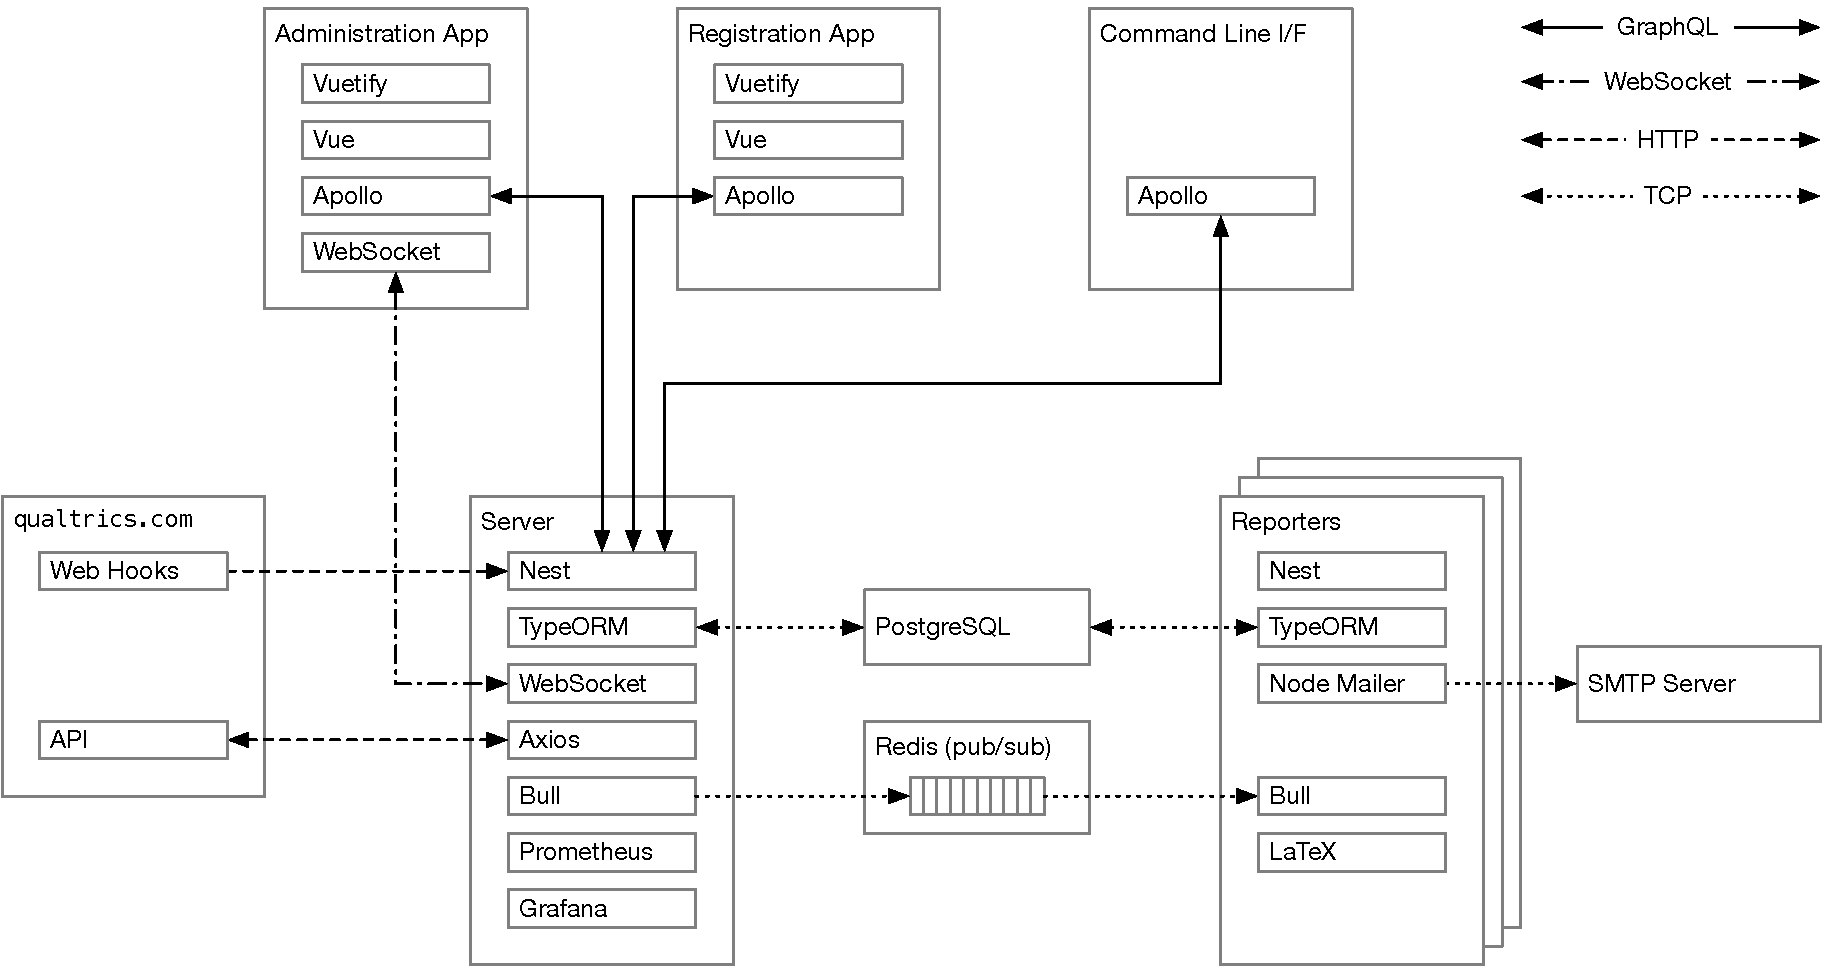
\includegraphics[width=\textwidth]{block-diagram}
  \caption{Block diagram of \caper.
    Communication between distributed processes is indicated in the legend.}
  \label{fig:block-diagram}
\end{figure}

\subsection{Data Model}
\label{sec:data-model}

Figure~\ref{fig:erd} shows the entity-relationship diagram for \caper's \pg{} database.
\begin{figure}
  \centering
  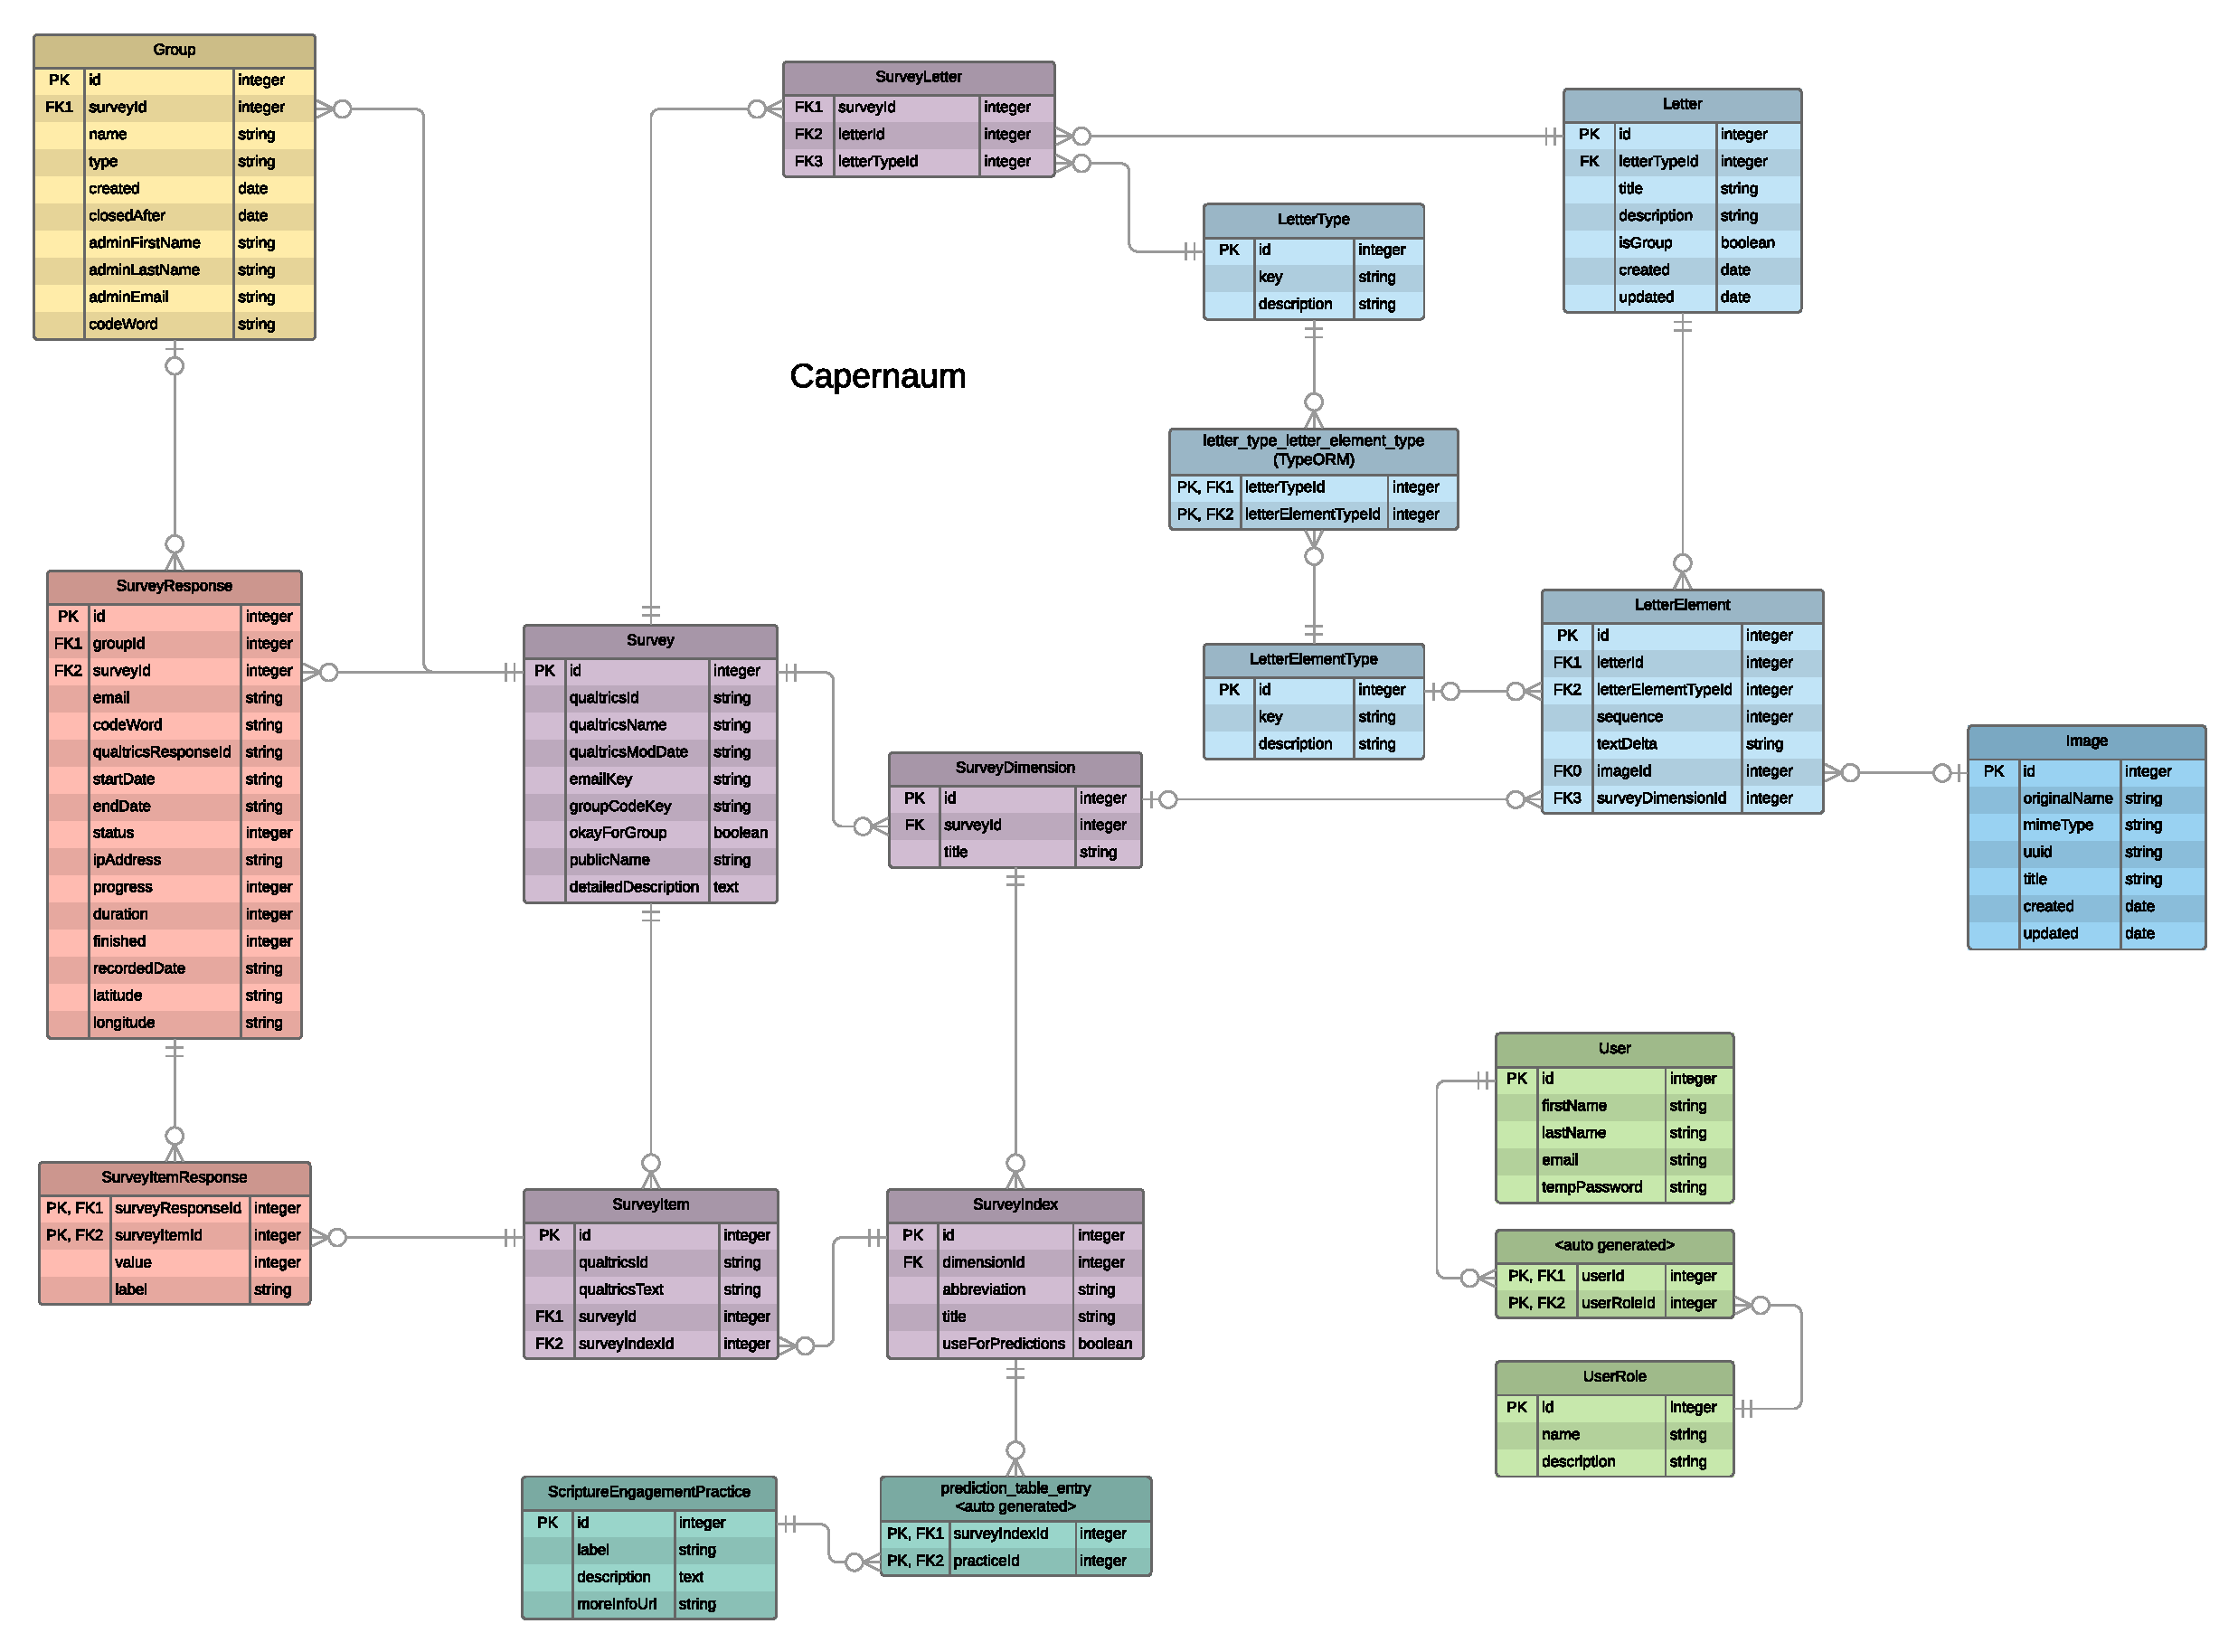
\includegraphics[width=\textwidth]{data-model}
  \caption{Entity-relationship diagram for \caper.}
  \label{fig:erd}
\end{figure}

\paragraph{\textcolor{Violet}{Surveys (violet)}}

The \texttt{Survey} and \texttt{SurveyItem} tables
capture the details of a single survey on \qual.
Using identifiers provided by \qual,
these tables allow \caper{} to perform the statistical analysis at the heart of each report letter.
To support statistical analysis,
\caper{} allows survey questions to be grouped into a category hierarchy.
Each survey question (\texttt{SurveyItem})
can be grouped into a \texttt{SurveyIndex},
which can in turn be grouped into a \texttt{SurveyDimension}.
\caper{} uses the latter entity to calculate aggregate attitudes
toward characteristics measured by the survey instrument itself.

\paragraph{\textcolor{Salmon}{Survey Responses (salmon)}}

The \texttt{SurveyResponse}
and \texttt{SurveyItemResponse}
tables store the responses a single respondent
makes to a survey.
\texttt{SurveyResponse} is related to a survey
and has one associated \texttt{SurveyItemResponse}
for each \texttt{SurveyItem}.

\paragraph{\textcolor{LightBlue}{Letters (light blue)}}

Reports sent to survey respondents are called ``letters'' in the data model.
Report content is entirely data driven and can be updated by a \caper's administrative user
as desired for new surveys, new versions of a survey, or new report formats.

Each \texttt{Letter} contains multiple
instances of a \texttt{LetterElement}.
A \texttt{LetterElement} has an associated type
(e.g., boilerplate text,
uploaded image,
graph of analytical results).

\caper{} can report results for individual survey respondents
and can also aggregate results for people who identify as part of a group.
The \texttt{LetterType} entity enforce this distinction
and also partitions the types of letter elements,
allowing the user interface to present only valid \emph{element} types
for each \emph{letter} type.

\paragraph{\textcolor{Goldenrod}{Groups (gold)}}

Survey respondents can indicate membership in a group of respondents
(e.g., members of a church, students in a course).
Each \texttt{Group} entity stores the detail of one group
and will be associated with a \texttt{SurveyResponse}
when the respondent enters his or her group code
prior to taking the survey.

\paragraph{\textcolor{LightGreen}{Users (green)}}

Because only a few administrative users have a need to log into \caper{} itself,
its user management is quite modest.
There is a many-to-many relationship between \texttt{User} and \texttt{User Role},
allowing for conventional role-based access control.

A \texttt{User} authenticates with an email address and password.
Passwords are stored in encrypted form in the database.
One a user logs in,
access is granted using a
\href{https://jwt.io/}{JSON Web Token}
that enumerates each \texttt{UserRole} for which the \texttt{User} is authorized.

\texttt{UserRole} data are employed to control access to views
in the administrative application in the browser
as well as \gql{} and \rest{} API access on the server.

\subsection{Administrative Application}
\label{sec:admin-applications}

\caper{} includes a \vue{}- and \vuetify{}-based
``single-page''
administrative web app.
The principal user of the admin app
is a person tasked with using \caper{}
to analyze and report on \qual{} surveys.
It allows such a user to:
\begin{enumerate}
\item Download the details of a survey from \qual{},
  either for the first time or to update \caper{} after a change is made to the survey on \qual.
\item Create or edit a report (``letter'') to be associated with a survey.
  The app provides a convenient drag-and-drop interface
  that allows the user to add, remove, and rearrange the various type of
  letter elements to be included in the report sent to survey respondents.
\item Upload and curate images to be used in report letters.
\item View searchable data about survey responses gathered from \qual.
\item Manually trigger the creation and delivery of a report for a survey respondent
  for purposes of debugging or verification.
  
\end{enumerate}

\subsection{Registration Application}
\label{sec:group-application}

\subsection{Application Server}
\label{sec:application-server}

\subsection{Reporting Server}
\label{sec:reporting-server}

\subsection{Deployment}
\label{sec:deployment}

\caper{} employs a fully-automated deployment
using \href{https://www.ansible.com/}{Ansible}.
The \ghsrc{ansible/provision.yaml}{provisioning file} contains commands for \gh{}, OS updates, etc.

\end{document}

%%% Local Variables:
%%% mode: latex
%%% TeX-master: t
%%% End:

% LocalWords:  Ansible ansible Qualtrics nd lr SurveyItem SurveyIndex
% LocalWords:  SurveyDimension SurveyResponse SurveyItemResponse LightBlue
% LocalWords:  LetterElement LetterType
